\documentclass[12pt,letterpaper]{article}
\usepackage[utf8]{inputenc}
\usepackage[spanish]{babel}
\usepackage{graphicx}
\usepackage[left=2cm,right=2cm,top=2cm,bottom=2cm]{geometry}
\usepackage{graphicx} % figuras
% \usepackage{subfigure} % subfiguras
\usepackage{float} % para usar [H]
\usepackage{amsmath}
%\usepackage{txfonts}
\usepackage{stackrel} 
\usepackage{multirow}
\usepackage{enumerate} % enumerados
\renewcommand{\labelitemi}{$-$}
\renewcommand{\labelitemii}{$\cdot$}
% \author{}
% \title{Caratula}
\begin{document}

% Fancy Header and Footer
% \usepackage{fancyhdr}
% \pagestyle{fancy}
% \cfoot{}
% \rfoot{\thepage}
%

% \usepackage[hidelinks]{hyperref} % CREA HYPERVINCULOS EN INDICE

% \author{}
\title{Caratula}

\begin{titlepage}
\begin{center}
\large{UNIVERSIDAD PRIVADA DE TACNA}\\
\vspace*{-0.025in}
\begin{figure}[htb]
\begin{center}

\includegraphics[width=4cm]{./Imagenes/logo}
\end{center}
\end{figure}
\vspace*{0.15in}
INGENIERIA DE SISTEMAS  \\

\vspace*{0.5in}
\begin{large}
TEMA:\\
\end{large}

\vspace*{0.1in}
\begin{Large}
\textbf{Informe Sesión de Laboratorio Nro 02} \\
\end{Large}

\vspace*{0.3in}
\begin{Large}
\textbf{CURSO:} \\
\end{Large}

\vspace*{0.1in}
\begin{large}
INTELIGENCIA DE NEGOCIOS\\
\end{large}

\vspace*{0.3in}
\begin{Large}
\textbf{DOCENTE(ING):} \\
\end{Large}

\vspace*{0.1in}
\begin{large}
 Patrick Jose Cuadros Quiroga\\
\end{large}

\vspace*{0.2in}
\vspace*{0.1in}
\begin{large}
Integrantes: \\
\begin{flushleft}


Jorge Luis MAMANI MAQUERA    	           \hfill	(2016055236) \\


\end{flushleft}
\end{large}
\end{center}

\end{titlepage}

\section{Informe Power BI} 
\begin{flushleft}


\begin{itemize}
\textbf{Parte1: Resultados de Ventas Adventure Works }\\
\textbf{ }\\
  \item Paso 1: Resultados por medio de graficos de las tablas  Sales vSalesPerson y Sales.vStoreWithDemographics
\begin{center}
	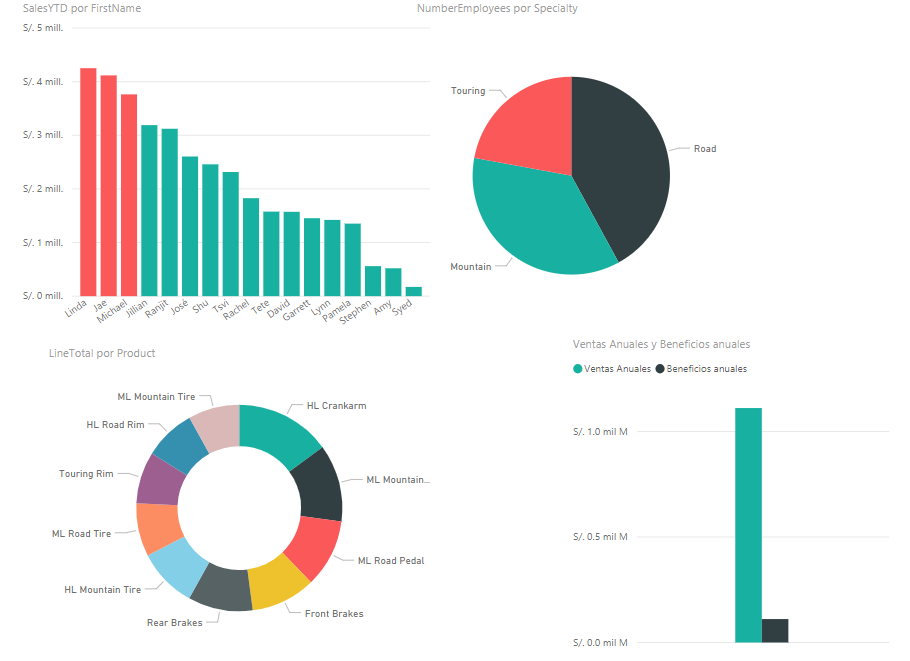
\includegraphics[width=20cm]{./Imagenes/resultado} 
	\end{center}


\textbf{ }\\
\textbf{ }\\
\textbf{ }\\
\textbf{ }\\
\textbf{ }\\
\textbf{ }\\
\textbf{ }\\
\textbf{ }\\
\textbf{ }\\
\textbf{ }\\

\textbf{Parte 2: Ruta del informe en el Portal de Power BI de los Resultados de Ventas Adventure Works }\\
\textbf{ }\\
  \item  https://app.powerbi.com/groups/me/reports/9590b0e7-a39d-42ee-887c-b900950de5b1/ReportSection

\end{itemize} 


\end{flushleft}
\end{document}